\documentclass{article}

\usepackage{xcolor}
\usepackage{graphicx}
\usepackage{fancyvrb}
\usepackage{listings}
\usepackage[T1]{fontenc}
\usepackage{hyperref}
\usepackage{amsmath}

\definecolor{officegreen}{rgb}{0, 0.5, 0}
\definecolor{navy}{rgb}{0, 0, 0.5}
\definecolor{linecolor}{rgb}{0.5, 0.6875, 0.6875}
\definecolor{outputcolor}{rgb}{0.375, 0.375, 0.375}

\newcommand{\id}[1]{\textcolor{black}{#1}}
\newcommand{\com}[1]{\textcolor{officegreen}{#1}}
\newcommand{\inact}[1]{\textcolor{gray}{#1}}
\newcommand{\kwd}[1]{\textcolor{navy}{#1}}
\newcommand{\num}[1]{\textcolor{officegreen}{#1}}
\newcommand{\ops}[1]{\textcolor{purple}{#1}}
\newcommand{\prep}[1]{\textcolor{purple}{#1}}
\newcommand{\str}[1]{\textcolor{olive}{#1}}
\newcommand{\lines}[1]{\textcolor{linecolor}{#1}}
\newcommand{\fsi}[1]{\textcolor{outputcolor}{#1}}
\newcommand{\omi}[1]{\textcolor{gray}{#1}}

% Overriding color and style of line numbers
\renewcommand{\theFancyVerbLine}{
\lines{\small \arabic{FancyVerbLine}:}}

\lstset{%
  backgroundcolor=\color{gray!15},
  basicstyle=\ttfamily,
  breaklines=true,
  columns=fullflexible
}

\title{Welcome to FsLab journal}
\date{}

\begin{document}

\maketitle



FsLab journal is a simple Visual Studio template that makes it easy to do 
interactive data analysis using F\# Interactive and produce nice HTML or PDF 
to document you research.
\subsection*{Next steps}

\begin{itemize}
\item 

To learn more about FsLab Journal, go to "Solution Explorer", right click
on your newly created project, select "Add", "New item.." and choose
"FsLab Walkthrough" (if you do not have R statistics environment installed)
or "FsLab Walkthrough with R" (if you do have R).

\item 

To add new experiments to your project, got to "Add", "New item" and choose
new "FsLab Experiment". You can have multiple scripts in a single project.

\item 

To see how things work, hit \textbf{F5} and see how FsLab Journal turns this
Markdown document with simple F\# script into a nice report!

\item 

To generate PDF from your experiments, you need to install \texttt{pdflatex} and 
have it accessible in the system \texttt{PATH} variable. Then you can run
\texttt{build pdf} in the folder with this script (then check out \texttt{output} folder).

\end{itemize}

\subsection*{Sample experiment}



We start by referencing \texttt{Deedle} and \texttt{FSharp.Charting} libraries and then we
load the contents of \emph{this} file:
\begin{Verbatim}[commandchars=\\\{\}, numbers=left]
\kwd{open} \id{Deedle}
\kwd{open} \id{System}\ops{.}\id{IO}
\kwd{open} \id{FSharp}\ops{.}\id{Charting}

\kwd{let} \id{file} \ops{=} \kwd{\_\_SOURCE\_DIRECTORY\_\_} \ops{+} \str{"}\str{{\textbackslash}{\textbackslash}}\str{Tutorial}\str{.}\str{fsx}\str{"}
\kwd{let} \id{contents} \ops{=} \id{File}\ops{.}\id{ReadAllText}(\id{file})
\id{printfn} \str{"}\str{Loaded}\str{ }\str{'}\str{\%}\str{s'}\str{ }\str{of}\str{ }\str{length}\str{ }\str{\%}\str{d}\str{"} \id{file} \id{contents}\ops{.}\id{Length}
\end{Verbatim}

\begin{lstlisting}
Loaded 'C:\Projects\github.com\sgoguen\sgoguen.github.com\Journal\Tutorial.fsx' of length 2247
\end{lstlisting}



Now, we split the contents of the file into words, count the frequency of 
words longer than 3 letters and turn the result into a Deedle series:
\begin{Verbatim}[commandchars=\\\{\}, numbers=left]
\kwd{let} \id{words} \ops{=} 
  \id{contents}\ops{.}\id{Split}(\str{' '}, \str{'"'}, \str{'{\textbackslash}n'}, \str{'{\textbackslash}r'}, \str{'*'})
  \ops{|>} \id{Array}\ops{.}\id{filter} (\kwd{fun} \id{s} \kwd{->} \id{s}\ops{.}\id{Length} \ops{>} \num{3})
  \ops{|>} \id{Array}\ops{.}\id{map} (\kwd{fun} \id{s} \kwd{->} \id{s}\ops{.}\id{ToLower}())
  \ops{|>} \id{Seq}\ops{.}\id{countBy} \id{id}
  \ops{|>} \id{series}
\end{Verbatim}



Finally, let's build a chart showing the top 6 words occuring in this tutorial:
\begin{Verbatim}[commandchars=\\\{\}, numbers=left]
\id{words} 
\ops{|>} \id{Series}\ops{.}\id{sort}
\ops{|>} \id{Series}\ops{.}\id{rev}
\ops{|>} \id{Series}\ops{.}\id{take} \num{6}
\ops{|>} \id{Chart}\ops{.}\id{Column}
\end{Verbatim}



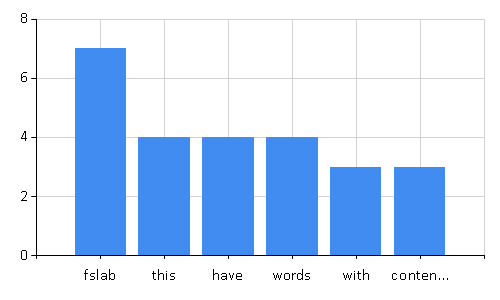
\includegraphics[width=1.0\textwidth]{./images/chart1.png}

\subsection*{Summary}



An image is worth a thousand words:


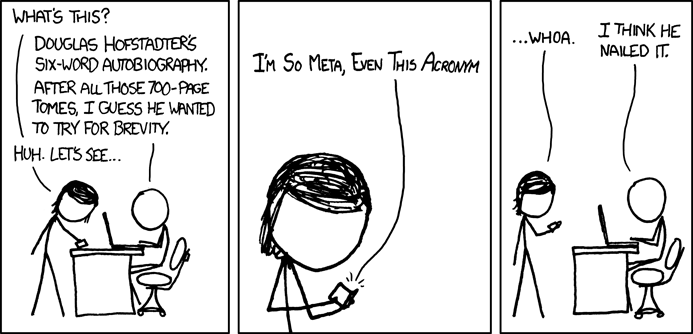
\includegraphics[width=1.0\textwidth]{./savedimages/saved1.png}





\end{document}
